%!TEX root = ../thesis.tex  % Comment this line for standalone compilation
%*******************************************************************************
%*********************************** First Chapter Appendix *****************************
%*******************************************************************************

\chapter{CAFLOW: Conditional Autoregressive Flows}  %Title of the First Chapter
\section{Architecture}

In this first section of the appendix, we provide more details about the architecture of the unconditional multi-scale flows and the conditional autoregressive multi-scale flows which comprise our modeling framework shown in Figure \ref{ch1:fig:high_level_design_conditional}.

\subsection{Unconditional multi-scale flows}\label{ch1:unconditional-architecture}
The sequence of transformations in each scale are:

\begin{enumerate}
    \item \textbf{Dequantization layer} (only in the first scale). Each pixel of each image channel admits an integer value from $0$ to $255$. If we do not modify those values, we model a high dimensional distribution in discrete space. However, normalizing flows rely on the rule of change of variables which is naturally defined in continuous space. Therefore, training a normalizing flow on the raw images will result in a model which which will place arbitrarily high likelihood on a few RGB values. This behavior leads to catastrophic destabilization of the training procedure and very poor performance. To remedy this problem, we convert the discrete space to continuous space by dequantizing each pixel value by resampling it from the distribution $q(u_{deq}|u)=\mathcal{U}([u,u+1))$, where $\mathcal{U}([u,u+1))$ is the uniform distribution over the interval $[u,u+1)$. This is called \textbf{uniform dequantization} and it is used by the majority of normalizing flow models in the literature. Dequantization effectively represents images as hypercubes. Modeling such sharp borders is challenging for a normalizing flow as it relies on smooth transformations. For this reason, \cite{ho2019flow++} proposed to learn the dequantization distribution $q(x_{deq}|x)$, where $x$ is the quantized and $x_{deq}$ the dequantized image using a conditional normalizing flow. This is called \textbf{variational dequantization}. We noticed that using variational dequantization results in a significant increase in performance. For this reason, we decided not to use variational dequantization in the experiments where we compare against other conditional flows, because this would defeat the purpose of fair comparison. We used variational dequantization in the experiments where we compare against methods which do not rely on normalizing flows.
    
    \item \textbf{Squeeze layer}. We squeeze the tensor in the channel dimension effectively halving the spatial resolution: the shape of the tensor is transformed from $(B, C, H, W)$ to $(B, 4C, H/2, W/2)$, where $B$ is the batch size, $C$ the number of channels, $H$ the height and $W$ the width of the image.
    \item \textbf{Two transition steps}. Each transition step consists of an invertible normalization layer (ActNorm) followed by an invertible $1\times 1$ convolution layer. According to \cite{SRFLOW}, the transition step allows the network to learn a linear invertible interpolation between neighboring pixels after the application of the squeeze layer. If the transition steps are not used, the squeeze layer may lead to checkerboard artifacts in the reconstructed image because it is exclusively based on pixel-reordering.
    \item \textbf{K flow steps}. Each flow step consists of an invertible normalization layer, invertible $1\times 1$ convolution layer and an affine coupling layer in that order. The scale and the bias in the affine coupling layer are computed by a simple convolutional neural network which performs three sequential convolutions with a $3\times 3$, $1\times 1$ and $3\times 3$ convolutional kernels respectively. The number of kernels in each convolutional layer is chosen to be $64$.
    \item \textbf{Split layer}. We split off half of the channels before the squeeze layer of the next scale. Therefore, the next scale transforms only the half part of the tensor. This motivates the modeling of variations in different resolutions and ultimately the hierarchical latent space decomposition of images using multi-scale normalizing flows. Empirically, it has been observed that the first split variables typically encode noise patterns or image details, while the final split variables encode higher level information.
    
\end{enumerate}
\newpage
\subsection{Conditional multi-scale flows}

Each scale of a conditional flow $F_i^{\theta}$ contains the following transformations in order:

\begin{enumerate}
    \item \textbf{Squeeze layer}.
    \item \textbf{Two transition steps}.
    \item \textbf{M Conditional flow steps}. We adopt the conditional flow step design used by \cite{SRFLOW}: \begin{enumerate}
        \item Invertible normalization (ActNorm).
        \item Invertible $1\times 1$ convolution.
        \item Affine injector.
        \item Conditional affine coupling layer.
    \end{enumerate}
    \item \textbf{Split layer}.
\end{enumerate}


We calculate the scale and the bias of the affine transformations in the affine injector and the conditional affine coupling layer using the same convolutional neural network as the one we used for the unconditional flows. The only difference is that we use $32$ instead of $64$ kernels.

\newpage

\section{Hierarchical Representation in Multi-Scale Normalizing Flows}\label{ch1:Hierarchical-Representation-in-Multi-Scale-Normalizing-Flows}

One of the fundamental advantages of employing a multi-scale architecture within normalizing flows lies in its capability to capture latent factors across various levels of abstraction. This phenomenon, where deeper layers tend to encapsulate higher-level information while earlier layers capture finer-grained details, can be attributed to the interplay of two key factors: the depth of computation and the imposed information bottleneck.

The depth of computation factor refers to the fact that in a multi-scale normalizing flow, computation occurs layer by layer, with each layer gradually refining the representation of the input data. When random noise is injected near the flow's output (in the reverse or generative order), most of the computation has already occurred. Consequently, this injected noise primarily influences the remaining local intricacies, such as fine-scale textures or subtle variations in the data. With fewer layers remaining to process, it becomes unlikely for this noise to introduce significant structural alterations or introduce entirely new objects into the scene.

The information bottleneck effect is closely linked to the architectural design of multi-scale normalizing flows, which involves latent space compression in the deeper layers of the normalizing flow.

The presence of this information bottleneck, combined with the depth of computation, compels the network to encode critical information at the deeper layers which don't have enough capacity to represent fine-grained details and simultaneously encode information that is used for the majority of the computation in the flow. Consequently, the network inclines toward prioritizing the encoding of high-level information, such as object identities or overarching scene attributes, within the deeper latent variables.

In essence, the multi-scale architecture's ability to model different levels of abstraction stems from the sequential nature of computation, where each layer refines the representation, and the imposed information bottleneck, which encourages the network to encapsulate essential, high-level details in deeper layers due to their restricted capacity for fine-grained representations.
\color{black}

\section{Details of experiments}\label{ch1:sec:details-of-experiments}
We used the same learning rate scheduling system for all experiments. Initially, we increase the learning rate linearly from $0$ to the target learning rate (usually $10^{-3}$) in the first $500$ iterations. Then, we use the pytorch STEPLR learning rate scheduler with value $\gamma = 0.999$. When the training curve levels-off (around $70$K iterations), we reduce the learning rate by a factor of $10$ until final convergence. This reduction provides a final performance boost. We do not repeat that reduction because it only results in overfitting. 

Moreover, we used exponential moving average (EMA) with a rate equal to $0.999$ in all experiments. We empirically found that EMA consistently provides a small increase in performance. Finally, we clipped the norm of the computed gradients to $1$, because it improved training stability with no noticeable compromise on performance. \\
 We adopted the hyperparameter values from the successful approaches in related work, as cited in \cite{Dual-Glow}. Due to the computational intensity of training normalizing flows, hyperparameter tuning becomes computationally prohibitive.\color{black}


Our primary objective was to demonstrate that our proposed model, which employs auto-regressive conditional components, offers improved modelling flexibility compared to non-autoregressive conditional flows like CINN and DualGlow while maintaining computational efficiency. To ensure a fair comparison, we designed our model to have a parameter count that closely aligns with those of the conditional normalizing flow models we referenced. While the GAN-based models also have a similar parameter magnitude, we did not aim for a very close match since our main focus is on contrasting our method with other normalizing flow alternatives.
\color{black}

\subsection{Image super-resolution}
We used $3$ scales, $16$ flow steps in each level of the conditioning flow $R^\theta$, $32$ flow steps in the each level of the conditioned flow $T^\theta$ and $12$ conditional flow steps in each level of each conditional flow $F_i^{\theta}$. We set the regularization constant $\lambda = 0.01$. Moreover, we used variational dequantization implemented with a conditional flow of $4$ conditional flow steps, because we compared our method against methods which are not based on flows. We trained our model for $4.5$ days on a single NVIDIA TESLA P100 GPU on $68$K images of the FFHQ dataset with a target learning rate of $10^{-3}$. We used $1000$ images for validation and $100$ images for testing.


\subsection{Image colorization}

We used $3$ scales, $24$ flow steps in each level of the conditioning flow $R^\theta$, $24$ flow steps in the each level of the conditioned flow $T^\theta$ and $12$ conditional flow steps in each level of each conditional flow $F_i^{\theta}$. We set the regularization constant $\lambda = 0.01$. We used uniform dequantization as we intended to compare our method with \cite{ardizzone2019guided}, which is a conditional flow. We trained the model on $300$K images of the lsun bedroom dataset (this accounts for $10\%$ of the full dataset) on a single NVIDIA TESLA P100 GPU for 3 days with a target learning rate of $10^{-3}$. We used $1000$ validation images and $5000$ test images.

\subsection{Image inpainting}
We used $3$ scales, $30$ flow steps in each level of the conditioning flow $R^\theta$, $30$ flow steps in the each level of the conditioned flow $T^\theta$ and $16$ conditional flow steps in each level of each conditional flow $F_i^{\theta}$. We set the regularization constant $\lambda = 0.05$ and the target learning rate to $10^{-4}$, because we faced stability issues with smaller values of $\lambda$ and greater values of the target learning rate. We trained the model on $195$K images of the CelebA dataset for $5$ days on a single NVIDIA TESLA P100 GPU. We used 1000 images for validation and $2000$ images for testing. We used the same preprocessing as  \cite{cGLOW} and uniform dequantization.

\clearpage
\section{Visual results}\label{ch1:sec:extended-visual-results} %
\subsection{Image super-resolution}\ 
%%%%%%%%%%%%%%%

\begin{figure}[h!]
    \centering
    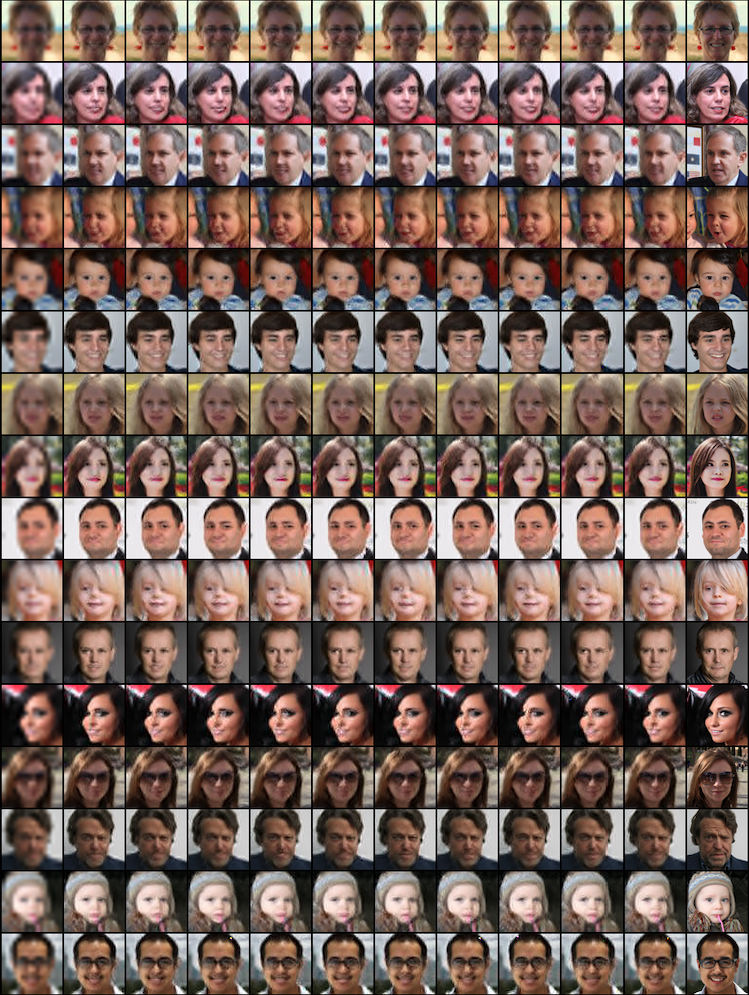
\includegraphics[width=0.8\textwidth]{Chapter1/paper_graphs/SupplementaryMaterial/ffhq_superresolved_2_0.5_cropped.png}
    \caption{Image super-resolution on the FFHQ dataset. Left: LR bicubicly upsampled. Right: HR image. Middle: 10 super-resolved versions in decreasing conditional log-likelihood order from left to right. We sampled 20 super-resolved images for each LR image and we present the 10 images with the highest conditional log-likelihood. We used sampling temperature $\tau=0.5$.}
\end{figure}

\clearpage

\begin{figure}[h!]
    \centering
    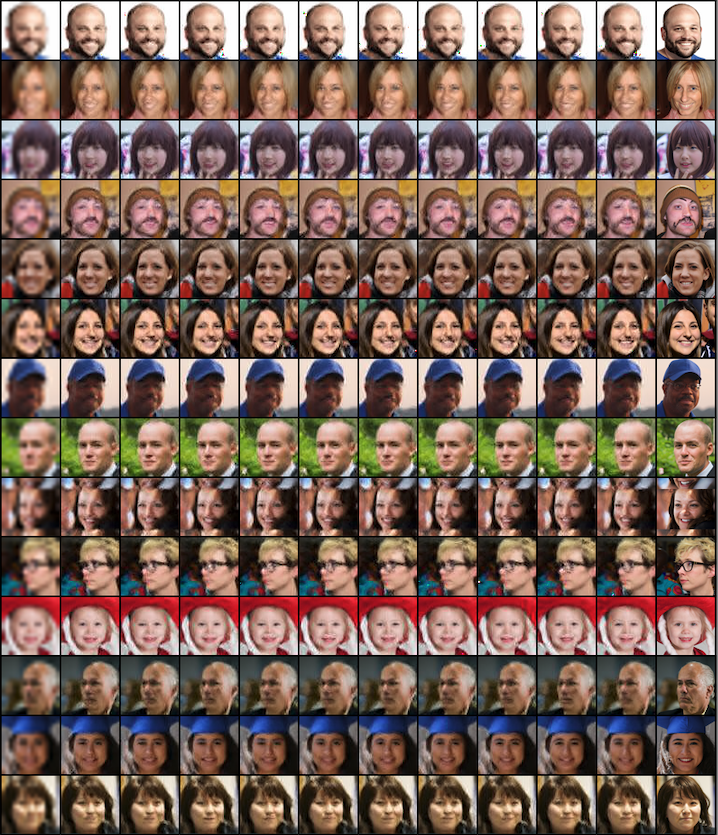
\includegraphics[width=\textwidth]{Chapter1/paper_graphs/SupplementaryMaterial/ffhq_super_0.55_0_cropped.png}
    \caption{Image super-resolution on the FFHQ dataset. Left: LR bicubicly upsampled. Right: HR image. Middle: 10 super-resolved versions in decreasing conditional log-likelihood order from left to right. We sampled 20 super-resolved images for each LR image and we present the 10 images with the highest conditional log-likelihood. We used sampling temperature $\tau=0.55$.}
\end{figure}

%inpainting
\clearpage
\subsection{Image inpainting}\ 
\begin{figure}[h!]
    \centering
    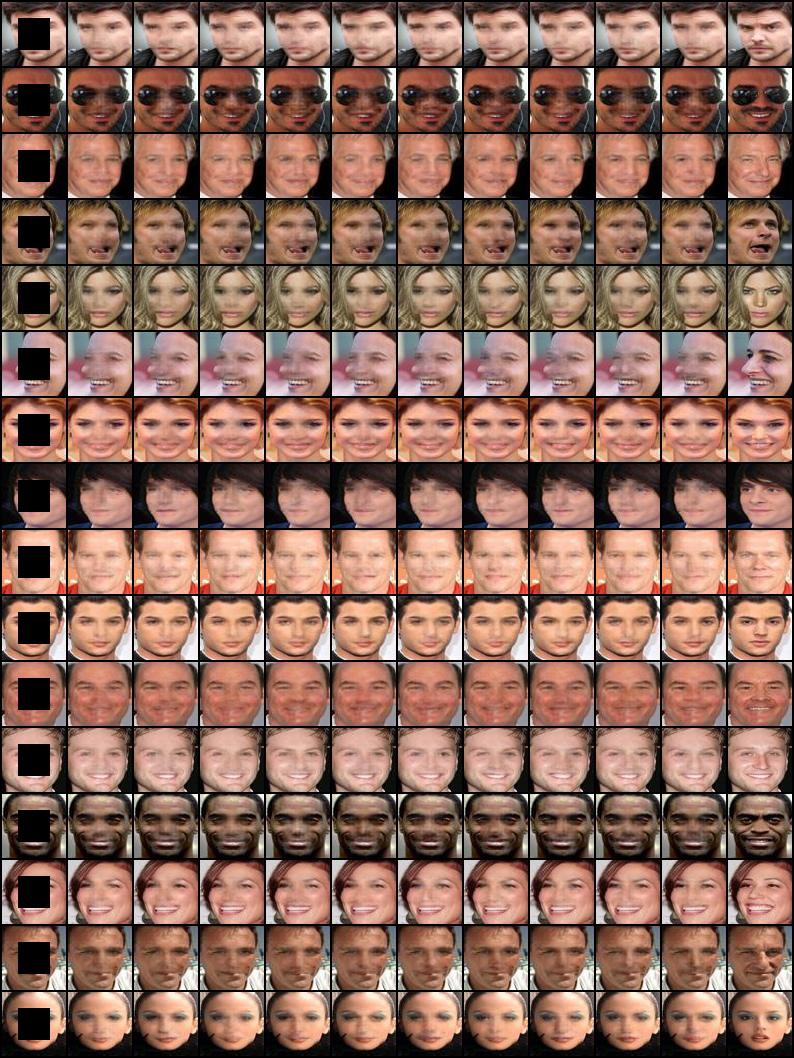
\includegraphics[width=0.8\textwidth]{Chapter1/paper_graphs/SupplementaryMaterial/inpainting_celebA_T_0.5_0.png}
    \caption{Image inpainting on the CelebA dataset. Left: Masked image. Right: Ground truth. Middle: 10 inpainted versions in decreasing conditional log-likelihood order from left to right. We sampled 30 inpainted images for each masked image and we present the 10 images with the highest conditional log-likelihood. We used sampling temperature $\tau=0.5$.}
\end{figure}

\begin{figure}[h!]
    \centering
    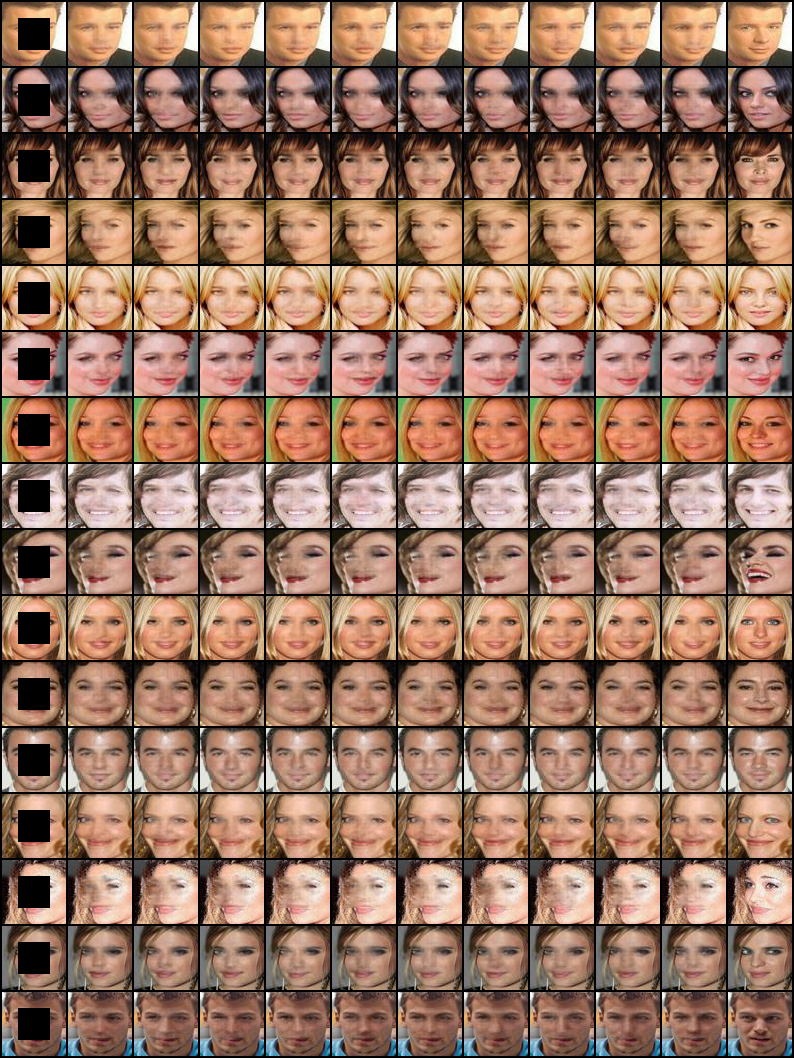
\includegraphics[width=\textwidth]{Chapter1/paper_graphs/SupplementaryMaterial/inpainting_celebA_T_0.5_1.png}
    \caption{Image inpainting on the CelebA dataset. Left: Masked image. Right: Ground truth. Middle: 10 inpainted versions in decreasing conditional log-likelihood order from left to right. We sampled 30 inpainted images for each masked image and we present the 10 images with the highest conditional log-likelihood. We used sampling temperature $\tau=0.5$.}
\end{figure}
\clearpage
%colorization
\subsection{Image colorization}\ 
\begin{figure}[h!]
    \centering
    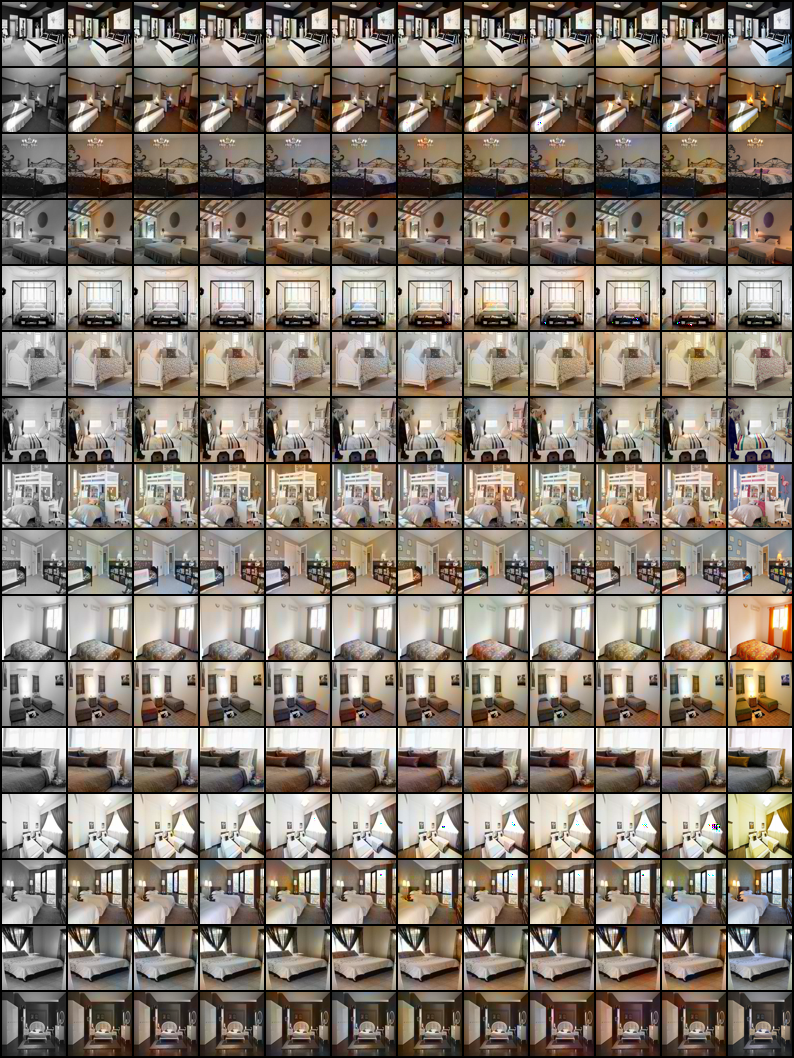
\includegraphics[width=0.8\textwidth]{Chapter1/paper_graphs/SupplementaryMaterial/colorisation_lsun_0.85.png}
    \caption{Image colorization on the LSUN BEDROOM dataset. Left: Grayscale image. Right: Ground truth. Middle: 10 colorized versions in decreasing conditional log-likelihood order from left to right. We sampled 25 colorized images for each greyscale image and we present the 10 images with the highest conditional log-likelihood. We used sampling temperature $\tau=0.85$.}
\end{figure}

\begin{figure}[h!]
    \centering
    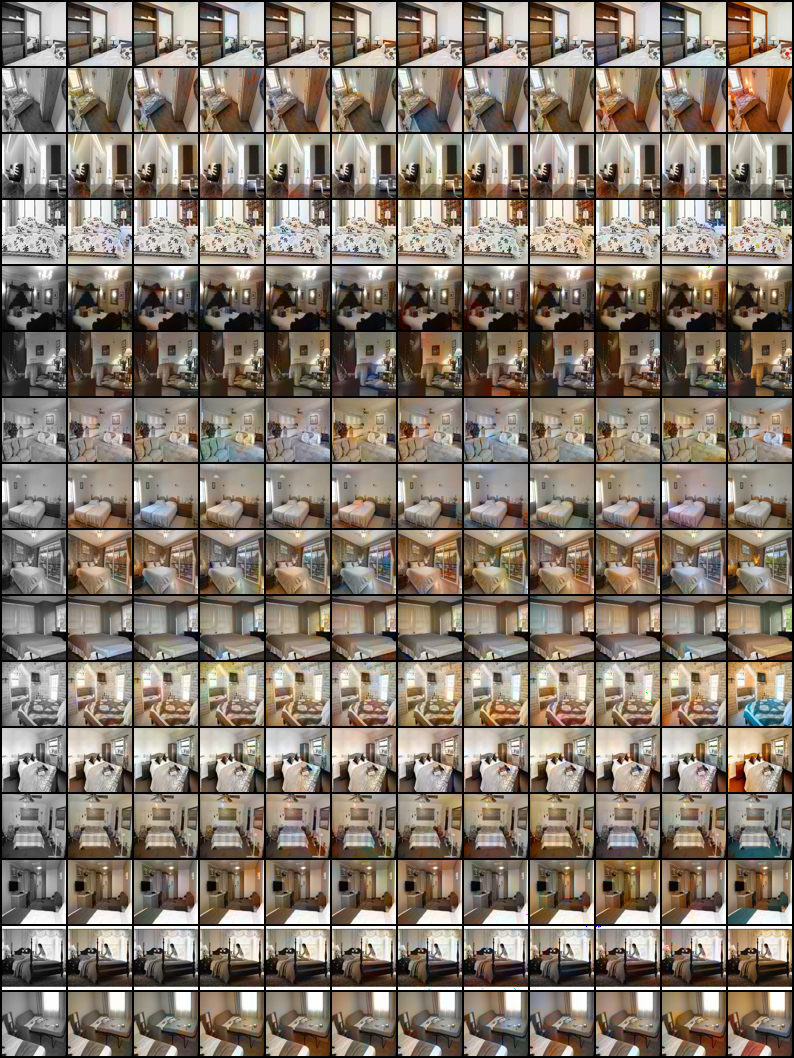
\includegraphics[width=\textwidth]{Chapter1/paper_graphs/SupplementaryMaterial/colorization_lsun_0.85_2.png}
    \caption{Image colorization on the LSUN BEDROOM dataset. Left: Grayscale image. Right: Ground truth. Middle: 10 colorized versions in decreasing conditional log-likelihood order from left to right. We sampled 25 colorized images for each greyscale image and we present the 10 images with the highest conditional log-likelihood. We used sampling temperature $\tau=0.85$.}
\end{figure}

\begin{figure}[h!]
    \centering
    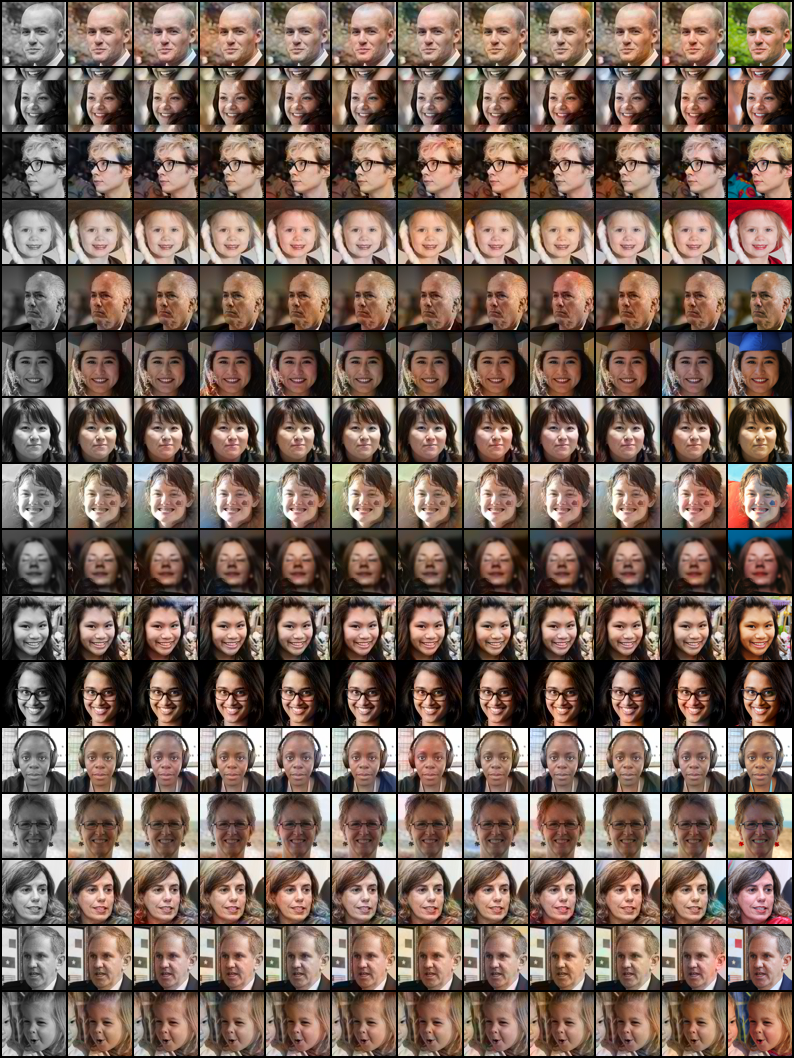
\includegraphics[width=\textwidth]{Chapter1/paper_graphs/SupplementaryMaterial/colorization_ffhq_T_0.7_0.png}
    \caption{Image colorization on the FFHQ dataset. Left: Grayscale image. Right: Ground truth. Middle: 10 colorized versions in decreasing conditional log-likelihood order from left to right. We sampled 25 colorized images for each greyscale image and we present the 10 images with the highest conditional log-likelihood. We used sampling temperature $\tau=0.7$.}
\end{figure}

\begin{figure}[h!]
    \centering
    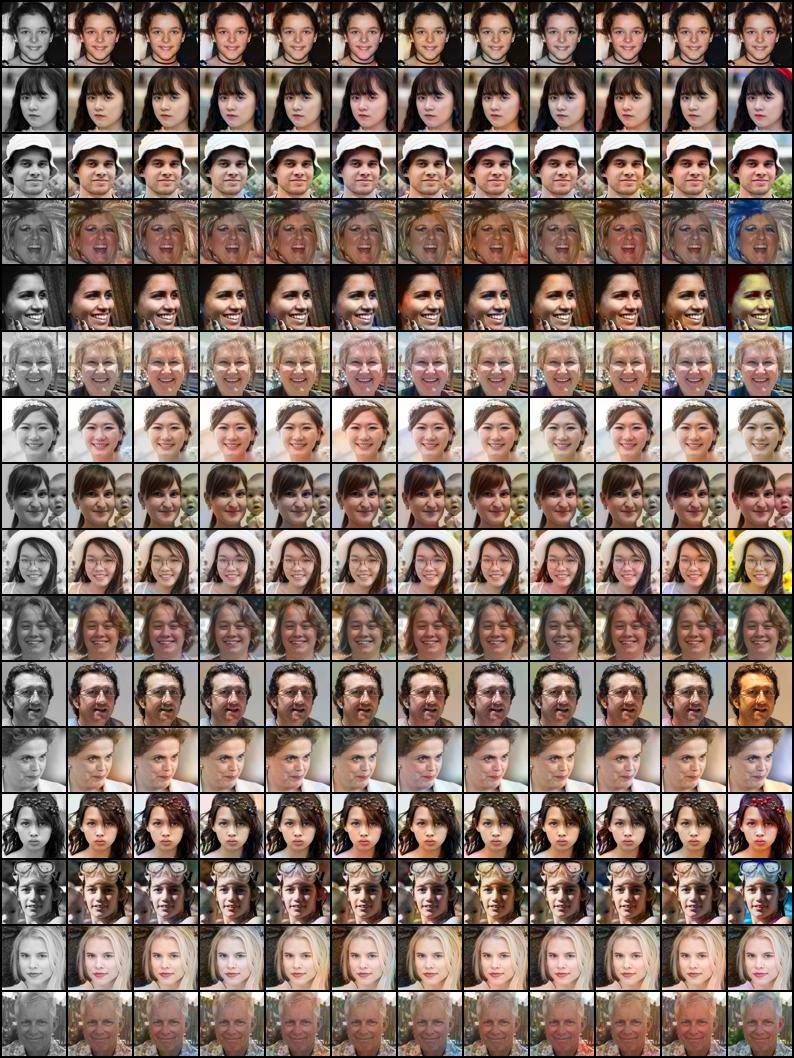
\includegraphics[width=\textwidth]{Chapter1/paper_graphs/SupplementaryMaterial/colorization_ffhq_0.7_1.png}
    \caption{Image colorization on the FFHQ dataset. Left: Grayscale image. Right: Ground truth. Middle: 10 colorized versions in decreasing conditional log-likelihood order from left to right. We sampled 25 colorized images for each greyscale image and we present the 10 images with the highest conditional log-likelihood. We used sampling temperature $\tau=0.7$.}
\end{figure}

\clearpage
\subsection{Sketch to image synthesis}\ 
\begin{figure}[h!]
    \centering
    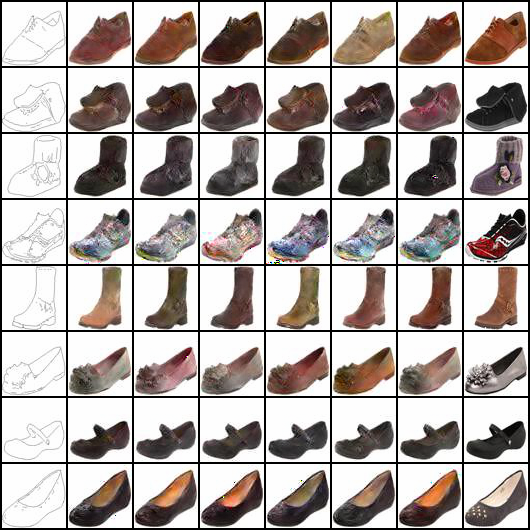
\includegraphics[scale=0.75]{Chapter1/paper_graphs/SupplementaryMaterial/edges2shoes_T_0.8.png}
    \caption{Sketch to image synthesis on the edges2shoes dataset \cite{isola2017image}. Left: Sketch. Right: Ground truth. Middle: 6 samples taken with sampling temperature $\tau=0.8$.}
\end{figure}